\documentclass{beamer}

% TODO: print out https://www.fuzzingbook.org/code/Intro_Testing.py

\usetheme{Boadilla}

%\includeonlyframes{current}

\usepackage{times}
\usefonttheme{structurebold}
\usepackage{listings}

\usepackage{pgf}
\usepackage{tikz}
\usepackage{alltt}
\usepackage[normalem]{ulem}
\usetikzlibrary{arrows}
\usetikzlibrary{automata}
\usetikzlibrary{shapes}
\usepackage{amsmath,amssymb}
\usepackage{rotating}
\usepackage{ulem}

\usetikzlibrary{arrows,automata,shapes}
\tikzstyle{block} = [rectangle, draw, fill=blue!20, 
    text width=5em, text centered, rounded corners, minimum height=2em]
\tikzstyle{bt} = [rectangle, draw, fill=blue!20, 
    text width=4em, text centered, rounded corners, minimum height=2em]

\lstdefinelanguage{JavaScript}{
  keywords={typeof, new, true, false, catch, function, return, null, catch, switch, var, if, in, while, 
do, else, case, break},
  keywordstyle=\color{blue}\bfseries,
  ndkeywords={class, export, boolean, throw, implements, import, this},
  ndkeywordstyle=\color{darkgray}\bfseries,
  identifierstyle=\color{black},
  sensitive=false,
  comment=[l]{//},
  morecomment=[s]{/*}{*/},
  commentstyle=\color{purple}\ttfamily,
  stringstyle=\color{red}\ttfamily,
  morestring=[b]',
  morestring=[b]''
}

%\setbeamercovered{dynamic}
\setbeamertemplate{footline}[page number]{}
\setbeamertemplate{navigation symbols}{}
\usefonttheme{structurebold}

\title{Software Testing, Quality Assurance \& Maintenance---Lecture 4}
\author{Patrick Lam\\University of Waterloo}
\date{January 15, 2025}

\colorlet{redshaded}{red!25!bg}
\colorlet{shaded}{black!25!bg}
\colorlet{shadedshaded}{black!10!bg}
\colorlet{blackshaded}{black!40!bg}

\colorlet{darkred}{red!80!black}
\colorlet{darkblue}{blue!80!black}
\colorlet{darkgreen}{green!80!black}

\newcommand{\rot}[1]{\rotatebox{90}{\mbox{#1}}}
\newcommand{\gray}[1]{\mbox{#1}}

\newenvironment{changemargin}[1]{% 
  \begin{list}{}{% 
    \setlength{\topsep}{0pt}% 
    \setlength{\leftmargin}{#1}% 
    \setlength{\rightmargin}{1em}
    \setlength{\listparindent}{\parindent}% 
    \setlength{\itemindent}{\parindent}% 
    \setlength{\parsep}{\parskip}% 
  }% 
  \item[]}{\end{list}}



\begin{document}

\usebackgroundtemplate{\tikz\node[opacity=0.1]{
\includegraphics[width=\paperwidth]{L02/07172_about_banmochi_ishi_strength_and_grip_testing.JPG}};}
\begin{frame}
  \titlepage
\end{frame}

\part{When to stop? \\ Idea 2: Mutation Analysis}
\begin{frame}
  \partpage
\end{frame}

\usebackgroundtemplate{\tikz\node[opacity=0.3]{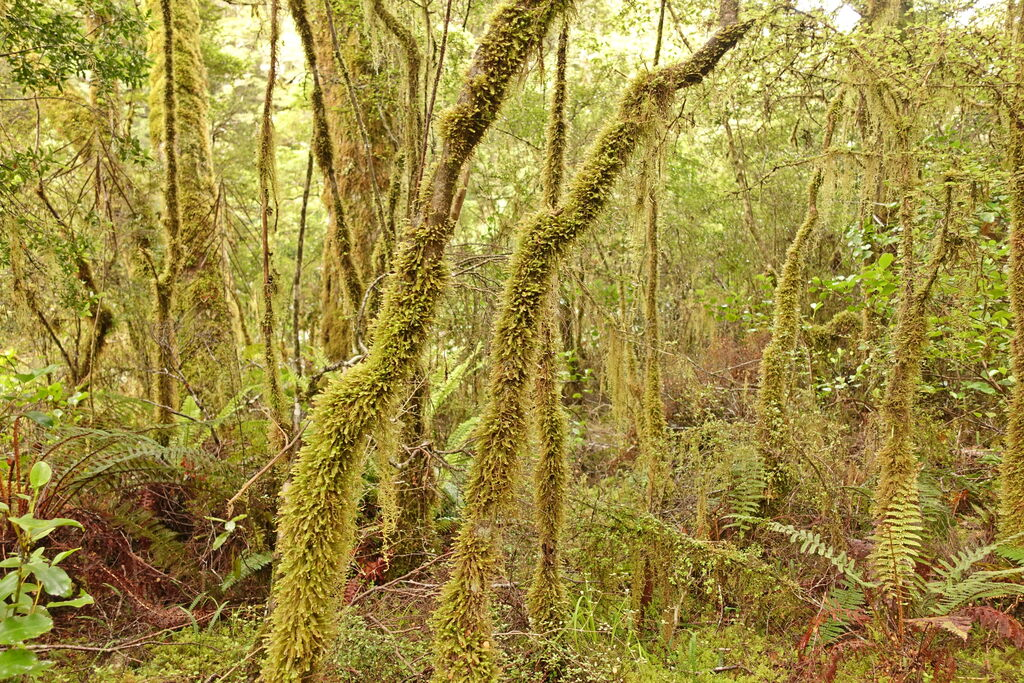
\includegraphics[width=\paperwidth]{L03/09038_lots_of_moss_v1.JPG}};}
\begin{frame}
  \frametitle{How many tests?}
  \Large
  \begin{changemargin}{2em}
    Do you have enough tests? How do you know?\\[1em]

    Let's fuzz the test suite.\\
    ~~ How? Modifying the program and seeing if the test suite notices.
  \end{changemargin}
\end{frame}

\usebackgroundtemplate{\tikz\node[opacity=0.3]{
\includegraphics[width=\paperwidth]{L04/20241110_001424746_blackbird.jpg}};}
\begin{frame}
  \frametitle{Mutants}
  \Large
  \begin{changemargin}{2em}
    A \alert{mutant} is a modified version of the program being tested.\\[1em]
    Usually we change an operator or identifier:
    \[ x + 5 \Rightarrow x - 5 \]
    
  \end{changemargin}
\end{frame}

\usebackgroundtemplate{}
\begin{frame}
  \frametitle{Killing Mutants}
  \Large
  \begin{changemargin}{2em}
    The test suite should fail on the mutant. \\
    Then the mutant is \alert{killed}.\\[1em]

    Remember: arrange, act, assert.\\
    Mutant might trigger errors during act;\\
    or it may detect different output during assert.
  \end{changemargin}
\end{frame}

\begin{frame}[fragile]
  \frametitle{Example Mutants}
  \begin{changemargin}{2em}
    Use language grammar to create mutants (code/L04/minval.c).\\[1em]
  \end{changemargin}
  \small
\begin{minipage}[t]{.4\textwidth}
\begin{alltt}
// original
int min(int a, int b)
\{
  int minVal;
  minVal = a;

  if (b < a) \{


    minVal = b;



  \}
  return minVal;
\}
\end{alltt}
\end{minipage} \begin{minipage}[t]{.4\textwidth}
\begin{alltt}
// with mutants
int min(int a, int b)
\{
  int minVal;
  minVal = a;
  minVal = b;               // \(\Delta 1\)
  if (b < a) \{
  if (b > a) \{              // \(\Delta 2\)
  if (b < minVal) \{         // \(\Delta 3 \)
    minVal = b;
    BOMB();                 // \(\Delta 4\)
    minVal = a;             // \(\Delta 5\)
    minVal = failOnZero(b); // \(\Delta 6\)
  \}
  return minVal;
\}
\end{alltt}
\end{minipage}
  
\end{frame}

\begin{frame}[fragile]
  \frametitle{Testing on the mutants}

  \begin{changemargin}{2em}
    Here's a test suite. How do the mutants do? \\[1em]
\begin{tabular}{lcccccc}
  & $\Delta$ 1 & $\Delta$ 2 & $\Delta$ 3 & $\Delta$ 4 & $\Delta$ 5 & $\Delta$ 6\\ 
  $\langle a = 0, b = 1, \mathrm{exp} = 0 \rangle$   & kill & & -- \\
  $\langle a = 1, b = 0, \mathrm{exp} = 0 \rangle$   & --   & & -- \\
  $\langle a = 1, b = 1, \mathrm{exp} = 1 \rangle$   &      & & -- \\
  $\langle a = 1, b = 349, \mathrm{exp} = 1 \rangle$ &      & & -- \\
\end{tabular}

~\\
Observe: $\Delta 3$ not killable.
    
  \end{changemargin}
\end{frame}

\begin{frame}
  \frametitle{Key idea for Mutation Analysis}
  \Large
  \begin{changemargin}{2em}
    Idea: use mutation analysis to evaluate test suite quality/improve test suites.\\[1em]
    Good test suites ought to be effective at killing mutants.
  \end{changemargin}

\end{frame}


\begin{frame}
  \frametitle{Why should this work? (1/2)}

    \Large
    \begin{changemargin}{2em}
      \alert{Competent Programmer Hypothesis}: \\
      \hspace*{2em}programmers usually are almost right,\\
      \hspace*{2em}except for ``subtle, low-level faults''.\\[1em]
      Mutation analysis tries to mimic this. (Exceptions?)
  \end{changemargin}

\end{frame}

\begin{frame}
  \frametitle{Why should this work? (2/2)}

    \Large
    \begin{changemargin}{2em}
      \alert{Coupling Effect Hypothesis}: \\
      \hspace*{2em}complex faults are the result of \\
      \hspace*{2em} simple faults combining.\\[1em]
      Hence, detecting all simple faults will detect many complex faults.\\[2em]

      Implication: test suites that are good at ensuring program quality also good at killing mutants.
      
  \end{changemargin}

\end{frame}

\usebackgroundtemplate{\tikz\node[opacity=0.1]{
\includegraphics[width=\paperwidth]{L04/0207_gold_mask.JPG}};}
\begin{frame}
  \frametitle{Mutation analysis in context}

  \begin{changemargin}{2em}
    Hard to apply by hand, and automation is complicated.\\[1em]
    Mutation is a ``gold standard'' \\
    \hspace*{2em} against which to test other testing criteria.\\[1em]
    Consider test suite $T$ which ensures statement coverage. \\
    What does mutation analysis say about $T$?
\end{changemargin}
\end{frame}

\usebackgroundtemplate{}

\part{Using Mutation Analysis}
\begin{frame}
  \partpage
\end{frame}


\begin{frame}
  \frametitle{Using Mutation Analysis}

  \Large
  \begin{changemargin}{2em}
    Three steps:
    \begin{enumerate}
    \item Generate mutants\\ ~~~(usually with a tool)
    \item Execute mutants\\ ~~~(computationally expensive)
    \item Classify\\ ~~~(manual)
    \end{enumerate}
    ~\\
    Then, create new test cases to kill remaining mutants.
  \end{changemargin}
  
\end{frame}

\begin{frame}[fragile]
  \frametitle{Mutation Analysis Diagram}
  \begin{center}
    \small
\resizebox{\textwidth}{.8\textheight}{%
\begin{tikzpicture}[->,>=stealth',shorten >=1pt,auto,node distance=3cm,
                    text width=4em,
                    semithick,initial text=]
  \node[text width=6em] (p) {Program $P$};
  \node[block,right of=p] (create) {Create mutants $m$};
  \node[block,right of=create] (elim) {Eliminate known-equivalent mutants};
  \node[block,right of=elim] (gen) {Generate test cases $T$};
  \node[block,right of=gen] (runTonP) {Run $T$ on $P$};
  \node[block,below of=runTonP,yshift=2em] (runTonM) {Run $T$ on all $M$};
  \node[block, below of=runTonM,yshift=2em] (filter) {Filter bogus mutants};
  \node[shape=ellipse, text centered, fill=blue!20, draw, text width=5em, left of=filter] (enough) {Enough mutants killed?};
  \node[block, left of=enough] (findThreshold) {Define threshold};
  \node[shape=ellipse, text centered, fill=blue!20, draw, text width=5em, below left of=enough,xshift=-10em] (correct) {Output of $p$ on $T$ correct?};
  \node[block, below of=correct,yshift=2em] (done) {Done};
  \node[block, below of=p,yshift=2em] (fixP) {Fix $P$};

  \path (p) edge node {} (create)
        (create) edge node {} (elim)
        (elim) edge node {} (gen)
        (gen) edge node {} (runTonP)
        (runTonP) edge node {} (runTonM)
        (runTonM) edge node {} (filter)
        (filter) edge node {} (enough)
        (findThreshold) edge node {} (enough)
        (correct) edge node {yes} (done)
        (fixP) edge node {} (p);
  \draw (correct) -| node[xshift=3em,yshift=2em] {no} (fixP); % no
  \draw (enough.north) -- node[xshift=2.5em] {no} (gen);
  \draw (enough) |- node[near start] {yes} (correct);
\end{tikzpicture}
}
\end{center}

\end{frame}

\begin{frame}
  \frametitle{Generating Mutants}

  \large
  \begin{changemargin}{2em}
    We said: mutation analysis is like fuzzing the test suite.\\
    Let's do that.\\[1em]

    \alert{Ground string}: A valid program (or fragment) that conforms to its grammar.\\[0.5em]
    \alert{Mutation operator}: A rule that specifies syntactic variations of strings.\\[0.5em]
    \alert{Mutant}: The result of one application of a mutation operator to a ground string.\\[1em]

    Workflow: parse the ground string (original program), apply a mutation operator, unparse.
  \end{changemargin}
\end{frame}

\begin{frame}
  \frametitle{Mutation Operators}

  \large
  \begin{changemargin}{2em}
    Hard to get good mutation operators.\\[1em]
    The $\Delta$s we saw applied operators: \\
    ~~~change identifiers, change operators, insert BOMB, insert failOnZero.\\[1em]
    Perhaps a bad operator: \\
    ~~~``change all boolean expressions to {\sf true}''.\\[1em]
    Research says: maybe (the right) 5 operators is enough.
    
  \end{changemargin}
\end{frame}

\begin{frame}
  \frametitle{When to Apply Mutation}

  \large
  \begin{changemargin}{2em}
    \begin{itemize}
    \item Once at a time, to a given ground string.
    \item Choose where to apply the operator randomly.
    \end{itemize}
  \end{changemargin}
\end{frame}

\begin{frame}
  \frametitle{Killing Mutants}

  \Large
  \begin{changemargin}{2em}
    One could define a mutation score \\~~~(\% of mutants killed),\\
    add tests until mutation score high enough.
  \end{changemargin}
\end{frame}

\begin{frame}
  \frametitle{HOWTO kill mutants}

  \Large
  \begin{changemargin}{2em}
    So far: need differences in \emph{output} (including assertion failures).\\[1em]
    Could relax to require changes in just the \emph{state}.

    \begin{itemize}
    \item strong mutation: fault must be reachable, infect state, and \emph{propagate} to output.
      \item weak mutation: fault must be reachable and infect state.
    \end{itemize}

    Supposedly: about the same in practice.
  \end{changemargin}
\end{frame}

\begin{frame}[fragile]
  \frametitle{Example 1}

  \begin{changemargin}{2em}
\begin{alltt}
// with mutants
int min(int a, int b)
\{
  int minVal;
  minVal = a;
  minVal = b;               // \(\Delta 1\)
  if (b < a) \{
    minVal = b;
  \}
  return minVal;
\}
\end{alltt}
~\\
Reachability: unavoidable; infection: $b \neq a$; \\
propagation: can't execute then case, so need $b > a$.\\[1em]
Strong mutation test case: $a = 5, b = 7$; \\
weak mutation: $a = 7, b = 5$.
  \end{changemargin}
\end{frame}


\begin{frame}[fragile]
  \frametitle{Example 2}

  \begin{changemargin}{2em}
\begin{alltt}
// with mutants
int min(int a, int b)
\{
  int minVal;
  minVal = a;
  if (b < a) \{
  if (b < minVal) \{         // \(\Delta 3 \)
    minVal = b;
  \}
  return minVal;
\}
\end{alltt}

~\\
This is an equivalent mutant, since \texttt{a = minVal};\\
infection condition is ``false''.\\[1em]

(Equivalence testing is generally undecidable.)
  \end{changemargin}
\end{frame}

\begin{frame}[fragile]
  \frametitle{Example 3}
\begin{minipage}{.5\textwidth} 
\begin{alltt}
  // original
  int foo(int x, int y) \{ 
  if (x > 5)
    return x + y;
  else
    return x;
  \}
\end{alltt}
\end{minipage}\begin{minipage}{.5\textwidth}
\begin{alltt}
  // mutant
  int foo(int x, int y) \{
  if (x > 5)
    return x - y;
  else
    return x;
  \}
\end{alltt}
\end{minipage}
\begin{changemargin}{2em}
  ~\\
  Test case $\langle 6,2 \rangle$ kills the mutant, while $\langle 6, 0 \rangle$ will not.\\[1em]
  Once we find a mutant-killing test case, forget the mutant and keep the test case (like fuzzing).
\end{changemargin}
\end{frame}

\begin{frame}
  \frametitle{Uninteresting Mutants}

  \large
  \begin{changemargin}{2em}
    Sometimes the mutant will loop indefinitely. Use a timeout.\\[1em]
    Other uninteresting mutants:
    \begin{itemize}
    \item stillborn: can't compile
    \item trivial: killed by any input
      \item equivalent
    \end{itemize}
  \end{changemargin}
\end{frame}

\begin{frame}
  \frametitle{Implementing Mutation Analysis}

  \large
  \begin{changemargin}{2em}
    What mutation analysis does:
    \begin{itemize}
    \item mimic (and hence test for) typical mistakes;
    \item encode knowledge re: specific kinds of effective tests: \\
      ~~e.g. statement coverage, checking for 0.
    \end{itemize}
    ~\\
    Choosing the right mutation operators is key.
  \end{changemargin}
\end{frame}

\begin{frame}
  \frametitle{Mutation Analysis Tool}

  \Large
  \begin{changemargin}{2em}
    PIT: \\
    \begin{center} {\large
      \url{https://pitest.org/quickstart/mutators/} } \\[1em]
    \end{center}
    Mutates your program, reruns your test suite, tells you how it went.\\[1em]
    Up to you: distinguish equivalent, not-killed.
    
  \end{changemargin}
\end{frame}

\begin{frame}[fragile]
  \frametitle{Exercise: Find Mutation Operators}

  \begin{changemargin}{2em}
\begin{lstlisting}
int mutationTest(int a, b) { 
  int x = 3 * a, y;
  if (m > n) {
    y = -n;
  }
  else if (!(a > -b)) {
    x = a * b;
  }
  return x;
}
\end{lstlisting}
  \end{changemargin}
  
\end{frame}

\begin{frame}[fragile]
  \frametitle{Exercise: Killing Mutants}

  \begin{changemargin}{2em}
    For the \texttt{mutationTest} code on the previous slide, find a test case to kill each of these types of mutants:\\[0.5em]
    \begin{itemize}
\item {\bf ABS}: Absolute Value Insertion\\
~~~{\tt x = 3 * a}
$\Longrightarrow$ {\tt x = 3 * abs(a)}\\[.5em]
\item {\bf ROR}: Relational Operator Replacement\\
~~~{\tt if (m > n)} $\Longrightarrow$ {\tt if (m >= n)}\\[.5em]
\item {\bf UOD}: Unary Operator Deletion\\
~~~{\tt if (!(a > -b))} $\Longrightarrow$ {\tt if (a > -b)}\\[.5em]
    \end{itemize}
  \end{changemargin}
\end{frame}


\begin{frame}
  \frametitle{Making Mutation Analysis Practical}

  \large
  \begin{changemargin}{2em}
  Petrović et al. ``Practical Mutation Testing at Scale: A View from Google''.\\[1em]

  Problems with mutation testing (aka mutation analysis):
  \begin{itemize}
  \item too many mutants!
  \item too many unproductive mutants!
  \end{itemize}
  \end{changemargin}
\end{frame}

\begin{frame}
  \frametitle{Practicality via Incrementality}
  \Large
  \begin{changemargin}{2em}
    Solution \#1: \\
    \qquad mutate only changed (and covered) lines of code; \\
    \qquad show surviving mutants during code review.
  \end{changemargin}
\end{frame}
  
\begin{frame}
  \frametitle{Mutation operators used}
  \Large
  \begin{changemargin}{2em}
    arithmetic operator replacement\\
    logical connector replacement\\
    unary operator insertion\\
    relational operator replacement\\
    statement block removal
  \end{changemargin}
\end{frame}

\begin{frame}
  \frametitle{Heuristics to avoid bad mutants: equivalent}
  \Large
  \begin{changemargin}{2em}
    \begin{itemize}
    \item detect some clearly-equivalent mutants
      (\texttt{c.size() == 0, c.size() <= 0})
    \item detect removal of caching
    \item detect time-related calls (e.g. sleep())
    \end{itemize}
  \end{changemargin}
\end{frame}

\begin{frame}
  \frametitle{Heuristics to avoid bad mutants: unproductive}
  \Large
  \begin{changemargin}{2em}
    Some mutants are killable but shouldn't be:
    \begin{itemize}
    \item logging calls
    \item mkdir
    \end{itemize}

    The test suite does not need to detect changes in logging output.
  \end{changemargin}
\end{frame}

\begin{frame}
  \frametitle{Applying mutation testing}
  \large
  \begin{changemargin}{2em}
    On a proposed change set:
    \begin{itemize}
    \item generate mutants for each changed line of code (max of 7x \# of files);
    \item filter out according to heuristics;
    \item probabilistically select mutants to choose those like past good mutants.
    \end{itemize}
    Developer should update their test sets accordingly.
  \end{changemargin}
\end{frame}

\part{Is Mutation Analysis Any Good?}
\begin{frame}
  \partpage
\end{frame}

\begin{frame}
  \frametitle{Paper: Are Mutants a Valid Substitute for Real Faults in Software Testing?}


  \begin{changemargin}{2em}
    \large
Answer: \alert{Yes!} Test suites
that kill more mutants are also better at finding real bugs. \\[1em]
Also identified types of bugs that then-current mutation analysis would not detect. \\[1em]

\scriptsize
Reference: René Just, Darioush Jalali, Laura Inozemtseva, Michael D. Ernst, Reid Holmes, and
Gordon Fraser. “Are Mutants a Valid Substitute for Real Faults in Software Testing?” In Foundations of Software Engineering 2014. pp654–665. \url{http://www.linozemtseva.com/research/2014/fse/mutant_validity/}\\[1em]
  \end{changemargin}
\end{frame}

\begin{frame}
  \frametitle{Mutation Effectiveness: Methodology}
  \Large
  \begin{changemargin}{2em}
    5 open-source projects.\\
    357 faults from these projects.\\
    230,000 mutants (using Major mutation framework).\\[1em]
    Can developer-written and automatically-generated test suites detect these faults?
  \end{changemargin}
\end{frame}

\begin{frame}[fragile]
  \frametitle{Mutation Effectiveness: Methodology}
  \begin{changemargin}{2em}
    For each fault:
    \begin{itemize}
    \item developer-written suite $T_{\mbox{bug}}$ that did not detect the fault;
    \item extracted from the source repo a developer-written test that detects the fault, add it to $T_{\mbox{bug}}$  to obtain $T_{\mbox{fix}}$.
    \end{itemize}
    Question: Does $T_{\mbox{fix}}$ detect more mutants than $T_{\mbox{bug}}$?\\
    If so, then the mutant behaves like a bug.

  \end{changemargin}
\end{frame}

\begin{frame}
  \frametitle{Results}
  \Large
  \begin{changemargin}{2em}
    Major-generated mutation could detect 73\% of the faults:\\
    ~~~that is, for 73\% of faults, some mutant will be killed by a test that also detects the fault.\\[1em]
    So: $\uparrow$ mutation coverage  also \\
    \hspace*{3em}$\uparrow$ likelihood of finding faults.\\[2em]
    
  \end{changemargin}
\end{frame}

\begin{frame}
  \frametitle{Results: Branch and Statement Coverage}
  \Large
  \begin{changemargin}{2em}
    Analogous numbers for branch and statement coverage: 50\%, 40\%.\\[1em]
    The 357 tests that find faults only increase branch coverage 50\% of the time.\\[1em]
    Improving your test suite doesn't get rewarded with a better coverage score.\\[1em]
    Conversely, improving statement coverage doesn't help find more bugs---you're not sensitive to erroneous state.
  \end{changemargin}
\end{frame}

\begin{frame}
  \frametitle{Results: Faults not found by mutants}
  \Large
  \begin{changemargin}{2em}
    27\% of remaining faults were not found by mutants.\\[1em]
    \begin{itemize}
    \item For 10\%, better mutation operators could have helped.
    \item Remaining 17\% not suitable for mutation analysis (algorithmic improvements or code deletion).
    \end{itemize}
  \end{changemargin}
\end{frame}
    

\begin{frame}
  \frametitle{Another Paper: Coverage is Not Strongly Correlated with Test Suite Effectiveness}

  \begin{changemargin}{2em}
  Reference: Laura Inozemtseva and Reid Holmes.
``Coverage is Not Strongly Correlated with Test Suite Effectiveness.''
In {\em International Conference on Software Engineering} 2014. pp435--445.
\url{http://www.linozemtseva.com/research/2014/icse/coverage/}
  \end{changemargin}

\end{frame}

\begin{frame}
  \frametitle{Coverage paper summary}

  \Large
  \begin{changemargin}{2em}
Coverage does not correlate with high quality
when it comes to test suites.\\[1em]

Specifically: test suites that are larger are better because
they are larger, not because they have higher coverage.
  \end{changemargin}
\end{frame}

\begin{frame}
  \frametitle{Methodology}

  \Large
  \begin{changemargin}{2em}
    5 large programs.\\
    Test suites: random subsets of developer-written suites.\\[1em]
    Measured coverage \& effectiveness (\%~mutants detected).
  \end{changemargin}

\end{frame}

\begin{frame}
  \frametitle{Result}

  \Large
  \begin{changemargin}{2em}
    After controlling for suite size, \\
    \hspace*{2em} coverage not strongly correlated \\
    \hspace*{2em} with effectiveness.\\[1em]
    Stronger coverage (e.g. branch vs statement) doesn't buy you better test suites.
  \end{changemargin}

\end{frame}

  
\end{document}
